\documentclass[output=paper]{langsci/langscibook}
\ChapterDOI{10.5281/zenodo.1407005}

\title{Why traces of the feminine survive where they do, in Oslo and Istria: How to circumvent some ``troubles with lexemes''}
\shorttitlerunninghead{Why traces of the feminine survive where they do, in Oslo and Istria}

\author{Hans-Olav Enger} 
 \abstract{The paper examines a surprising parallel in the development of the feminine \isi{gender} in Oslo Norwegian on the one hand and Istro-Romanian (spoken in Croatia) on the other. In both cases, the feminine \isi{gender} is lost on all `normal' \isi{gender} markers, but a trace of the feminine remains on the \isi{definite} \isi{suffix}, which is the `last redoubt' of the feminine \isi{gender}. An attempt is made to link this development to a slightly modified version of the \isi{Agreement Hierarchy}. It is suggested that the Hierarchy may be linked to \isi{grammaticalisation}, and that we should not draw too strict lines between different kinds of agreement.  }

\maketitle


\begin{document}
\selectlanguage{english}
\il{Norwegian|(}
\il{Istro-Romanian|(}

\section{The main point}

The starting-point for what follows is a parallel between Norwegian as
spoken in Oslo, Norway, and Istro-Romanian, as spoken on the Istrian
peninsula in Croatia. In both cases, feminine agreement is reduced,
diachronically, and in both cases, traces of the feminine remain longer
in one specific place, namely word-internally, than elsewhere. Why would
there be such a parallel? I suggest an account which involves a modified
version of %
%Corbett's (1979, 2006) 
\citeauthor{Corbett79}'s (\citeyear{Corbett79,Corbett2006}) %
%Corbett;Corbett
%
\isi{Agreement Hierarchy}. In brief, the
`\isi{definite} article', when it is a \isi{suffix}, has a different status than
other elements that signal \isi{gender}. Furthermore, Furthermore, an examination of the hierarchy reveals that it may be `anchored' in the workings of diachrony and
psycholinguistics.

\section{The empirical background}
\label{sec:enger:2.1}
\subsection{Oslo}

In the Oslo dialect of Norwegian, a change has taken place. A century
ago, this dialect had three genders\is{gender} (in the singular, like German).\footnote{The following draws on %
%Larsen (1907) 
\citet{Larsen1907} %
%Larsen
%
and %
%Lødrup (2011)
\citet{Lodrup11} 
  in particular; but cf. also %
%Enger (2004a, b) 
\citet{Enger2004a,Enger2004b} %
%Enger
%
and %
%Opsahl (2009)
\citet{Opsahl09}%
%Opsahl
%
.}
Compare (\ref{ex:Enger:1}):

\begin{exe}

\ex\label{ex:Enger:1} Three genders\is{gender} in Oslo dialect ca. 1900; examples in Norwegian Bokmål orthography.

\begin{xlist}
\ex\label{ex:Enger:1a}
\gll en liten gutt, en fin gutt, denne gutten, ikke noen gutt \\
a.\textsc{m} little.\textsc{m} boy, a.\textsc{m} fine.\textsc{mf} boy, this.\textsc{mf} boy.\textsc{def}.\textsc{sg}.\textsc{\{m\}}, not any.\textsc{m} boy \\

\ex\label{ex:Enger:1b}
\gll en liten stol, en fin stol, denne stolen, ikke noen stol \\
a.\textsc{m} little.\textsc{m} chair, a.\textsc{m} fine.\textsc{mf} chair, this.\textsc{mf} chair.\textsc{def}.\textsc{sg}.\textsc{\{m\}}, not any.\textsc{m} chair\\

\ex\label{ex:Enger:1c}
\gll ei lita jente, ei fin jente, denne jenta, ikke noa jente \\
a.\textsc{f} little.\textsc{f} girl, a.\textsc{f}. fine.\textsc{mf} girl, this.\textsc{mf} girl.\textsc{def}.\textsc{sg}.\textsc{\{f\}}, not any.\textsc{f} girl\\

\ex\label{ex:Enger:1d}
\gll ei lita jakke, ei fin jakke, denne jakka, ikke noa jakke \\
a.\textsc{f} little.\textsc{f} jacket, a.\textsc{f} fine.\textsc{mf} jacket, this.\textsc{mf} jacket.\textsc{def}.\textsc{sg}.\textsc{\{f\}}, not any.\textsc{f} jacket\\

\ex\label{ex:Enger:1e}
\gll et lite barn, et fint barn, dette barnet, ikke noe barn \\
a.\textsc{n} little.\textsc{n} child, a.\textsc{n} fine.\textsc{n} child, this.\textsc{n} child.\textsc{def}.\textsc{sg\{n\}}, not any.\textsc{n} child\\

\ex\label{ex:Enger:1f}
\gll et lite hus, et fint hus, dette huset, ikke noe hus \\
a.\textsc{n} small.\textsc{n} house, a.\textsc{n} fine.\textsc{n} house, this.\textsc{n} house.\textsc{def}.\textsc{sg\{n\}}, not any.\textsc{n} house\\
\end{xlist}
\end{exe}

There is clear evidence for three genders\is{gender}, masculine (\ref{ex:Enger:1a},\ref{ex:Enger:1b}), feminine
(\ref{ex:Enger:1c},\ref{ex:Enger:1d}) and neuter (\ref{ex:Enger:1e},\ref{ex:Enger:1f}). The formal differentiation between the
masculine and the feminine is not so clearly marked as that of both of
them in opposition to the neuter. The masculine--feminine distinction
is not realised on all associated words, but it is realised on some very
central determiners and a few highly frequent adjectives, such as the
adjective \emph{liten} `small', which is overdifferentiated;
showing `too many' contrasts %
%(cf. Corbett 2007)
\citep[cf.][]{Corbett2007}%
%Corbett
%
. By contrast, the
adjective \emph{fin} `fine' is `regular', showing only the opposition
neuter vs. non-neuter, in the same way as the proximal determiner
\emph{denne}.\footnote{There are also adjectives in which the \isi{gender}
  distinction does not show at all, e.g. \emph{rosa} `pink',
  \emph{gammaldags} `old-fashioned'.} In such cases, I have assigned the
value `mf'.

The status of the \isi{suffix} in the \isi{definite} singular of nouns is intriguing
%
(see e.g. %
%Enger \& Corbett 2012
\citealt{Enger12} %
%
 and \sectref{sec:enger:3.2.3} below)%
%\citep[see e.g. ][ and 3.2.3 below]{Enger12}%
%Enger-Corbett
%
. Genders\is{gender} are defined as
classes of nouns reflected in the behaviour of associated words %
%(Corbett 1991)
\citep{Corbett1991}%
%Corbett
%
. Suffixes\is{suffixation} do not count as `associated words'; and yet, in the
nouns in (\ref{ex:Enger:1}), the suffixes\is{suffixation} are in a strict 1:1 relation with the \isi{gender}
exponents. If a noun takes \emph{-a} in the \isi{definite} singular (e.g.
\emph{jente} `girl'), it will invariably also take \emph{ei}
`a.\textsc{f}'\emph{, lita} `little.\textsc{f}'\emph{, noa} `any.\textsc{f}' and other `associated
words' expected from a feminine: if it takes -\emph{en} in the \isi{definite}
singular, it will also take \emph{en} `a.\textsc{m}'\emph{, liten}
`small.\textsc{m}'\emph{, noen} `any.\textsc{m}', as expected from a masculine. This is
the background for the use of curly brackets in (\ref{ex:Enger:1}).

In Oslo these days, there is no longer any evidence from `associated
words' in favour of a separate feminine \isi{gender}. In other words, the
feminine agreement has been ousted by the old masculine. The old \isi{suffix}
\emph{-a}, by contrast, is retained. The system, at least for most of
the speakers, is as described in (\ref{ex:Enger:2}):

\ea\label{ex:Enger:2} Two genders\is{gender} in recent Oslo dialect (compare example \ref{ex:Enger:1}; again,
examples given in Bokmål)

\ea\label{ex:Enger:2a}
\gll {en liten gutt, en fin gutt, denne gutten, ikke noen gutt }\\
a.\textsc{m} small.\textsc{m} boy, a.\textsc{m} fine.\textsc{m} boy, this.\textsc{m} boy.\textsc{def}.\textsc{sg}.\textsc{\{m\}} not any.\textsc{m} boy\\

\ex\label{ex:Enger:2b}
\gll {en liten stol, en fin stol, denne stolen, ikke noen stol}\\
a.\textsc{m} small.\textsc{m} chair, a.\textsc{m} fine.\textsc{m} chair, this.\textsc{m} chair.\textsc{def}.\textsc{sg}.\textsc{\{m\}} not any.\textsc{m}
chair\\

\ex\label{ex:Enger:2c}
\gll {en liten jente, en fin jente, denne jenta, ikke noen jente}\\
a.\textsc{m} small.\textsc{m} girl, a.\textsc{m} fine.\textsc{m} girl, this.\textsc{m} girl.\textsc{def.sg.{\{}?{\}}} not any.\textsc{m}
girl\\

\ex\label{ex:Enger:2d}
\gll {en liten jakke, en fin jakke, denne jakka, ikke noen jakke}\\
a.\textsc{m} small.\textsc{m} jacket, a.\textsc{m} fine jacket, this.\textsc{m} jacket.\textsc{def}.\textsc{sg}.\textsc{{\{}?{\}}} not
any.\textsc{m} jacket\\

\ex\label{ex:Enger:2e}
\gll {et lite barn, et fint barn, dette barnet, ikke noe barn}\\
a.\textsc{n} small.\textsc{n} child, a.\textsc{n} fine.\textsc{n}. child, this.\textsc{n}
child.\textsc{def}.\textsc{sg}.\textsc{\{n\}} not any.\textsc{n} child\\

\ex\label{ex:Enger:2f}
\gll {et lite hus, et fint hus, dette huset, ikke noe hus}\\
a.\textsc{n} small.\textsc{n} house, a.\textsc{n} fine.\textsc{n} house, this.\textsc{neut}
house.\textsc{def}.\textsc{sg}.\textsc{\{n\}} not any.\textsc{n} house\\

\z
\z

The usual interpretation of the data in (\ref{ex:Enger:2}), as indicated by the
glossing, is that the old feminine is no longer a separate \isi{gender} in the
Oslo dialect, `merely' an inflection class %
%(Lødrup 2011, cf. also Enger
%2004a,b and many others)
(%
\citealt{Lodrup11}, cf. also \citealt{Enger2004a,Enger2004b} and many others)%
%\citep[, cf. also Enger 2004a,b and many others]{Lodrup11}%
%Lødrup
%
.\footnote{There is considerable discussion
  about whether to take pronouns into consideration for the purposes of
  \isi{gender} agreement. At this stage, they are left out, for expository
  reasons (but cf. \sectref{sec:enger:4.2} below).} The \isi{definite} singular~\isi{suffix} -\emph{a}
might seem `the last redoubt' of the old feminine, cf. (\ref{ex:Enger:2}c-d), and some
would like to analyse it is a \isi{gender} marker (cf. \sectref{sec:enger:3.2.3} below); that is
the reason for using ``\{?\}''.

A development from \isi{gender} to inflection class is far from unique; such
developments have been referred to as \isi{grammaticalisation} %
%(cf. Lehmann
%1982, 2016, Wurzel 1986)
\citep[cf.][]{Lehmann82,Lehmann16,Wurzel86}%
%Lehmann;Lehmann;?Wurzel
%
. The old feminine is changing into an
inflection class also in some other Norwegian dialects, such as Tromsø %
%(Westergaard \& Rodina 2015, 2016)
\citep{Westergaard15,Westergaard16}%
%
, and it is absent also in some
contact varieties in the North %
%(Conzett, Sollid \& Johansen 2011)
\citep{Conzett11}%
%Johansen
%
.
Essentially the same development is found in the Jämtland dialect in
Sweden %
%(van Epps \& Carling 2017)
\citep{VanEpps17}%
%
.\footnote{On the whole, it is
  pointless to debate whether dialects in Scandinavia are dialects of
  one or the other language, since Scandinavia generally counts as one
  dialect continuum. The point of interest is the parallel between
  Jämtland and Oslo.}\textsuperscript{,}\footnote{A next step after the
  system shown in (\ref{ex:Enger:2}) is that also the old -\emph{a} \isi{suffix} is lost. In
  that way, old masculines and old feminines become indistinguishable.
  This is found with some Oslo speakers, who will say \emph{en liten
  jakke, jakken,} just like \emph{en liten gutt,} \emph{gutten}.
  (Essentially the same system is found in ``standard'' \ili{Swedish} and
  \ili{Danish}.)}

\subsection{Istro-Romanian}

We now turn to Istro-Romanian, which is ``spoken in some localities in
north-eastern Istria (Croatia) to the south of Mt Učka, and in the town
of Žejane to its north. Its speakers probably descend from pastoral
communities originally resident in Bosnia, Serbia, and Croatia in the
late Middle Ages, who settled in Istria from about the fifteenth
century. The language's place of origin, and whether it originally broke
away from varieties spoken in the Romanian lands, or from those spoken
in the Balkans, or represents dialect mixing, remain controversial.
There are today perhaps 200-250 speakers in Croatia, mainly elderly and
all bilingual in Croatian'' %
%(Maiden 2016a: 91)
\citep[91]{Maiden16}%
%Maiden
%
.

The number of genders\is{gender} in Istro-Romanian might be disputed. The system
used to be essentially the same as that of \ili{Romanian}, and the number of
genders\is{gender} in \ili{Romanian} has been much disputed %
%(cf. Corbett 1991, Maiden
%2016b\&c, Loporcaro 2016)
\citep[cf.][]{Corbett1991,Maiden16b,Maiden16c,Loporcaro16}%
%Corbett;Maiden
%
. Besides the masculine and the feminine, which
are uncontroversial, there is also, at least according to %
%Corbett (1991)
\citet{Corbett1991} % 
%Corbett
%
and %
%Loporcaro (2016)
\citet{Loporcaro16}%
%Loporcaro
%
, a third \isi{gender}. This \isi{gender} has been referred to
as `neuter' and as `genus alternans'. This \isi{gender} has practically no
morphology of its own, as Table \ref{tab:Enger:romanian} shows.


\begin{table}
\begin{tabular}{lll}
\lsptoprule
Singular &  Plural & \\
\midrule
\emph{trandafir \textbf{frumos}}  & \emph{trandafiri frumoși} & (beautiful rose, M)\\
\emph{casa frumoasă}  & \emph{case frumo\textbf{ase}} & (beautiful house, F)\\
\emph{palton \textbf{frumos}} &  \emph{paltoane frumo\textbf{ase}} &
(beautiful coat, N)\\
\lspbottomrule
\end{tabular}
\begin{tabular}{llll}
\lsptoprule
\multicolumn{2}{c}{Singular with \isi{definite} article} &
\multicolumn{2}{c}{Plural with \isi{definite} article}\\
\midrule
\emph{pom - pom\textbf{ul}}
  & (tree - the tree, M)
  & \emph{pomii}
  & (the trees) \\
\emph{cutie - cutia}
  & (box - the box, F)
  & \emph{cutii\textbf{le }}
  & (the boxes) \\
\emph{loc - loc\textbf{ul}}
  & (place - the place, N)
  & \emph{locuri\textbf{le }}
  & (the places) \\
\lspbottomrule
\end{tabular}
\caption{\ili{Romanian} \isi{gender}.}
\label{tab:Enger:romanian}
\end{table}


The `neuter' patterns with the masculine in the singular, with the
feminine in the plural. Thus,
it alternates between the two, hence the label \emph{genus alternans}.
In Table~\ref{tab:Enger:romanian}, some endings have been boldfaced so as to show this. According
to Martin %
%Maiden
\citeauthor{Maiden16d}  (personal communication, and %
%
%2016d
\citeyear{Maiden16d}%
%
), in Istro-Romanian,
while the masculine and the feminine happily persist,

\begin{quote}
The plural endings which originally selected feminine \isi{gender}
(alternating with masculine singulars) have lost the alternating \isi{gender}
and the relevant nouns have become masculine in singular and plural
alike, \emph{\textbf{except}}~that they may continue to have a
\emph{\textbf{distinctively feminine}} \isi{definite} article (suffixed, as in Norwegian) \ldots{} this could indicate that the \isi{definite} article is in a
rather different category from other agreeing elements, at least when it
is enclitic to the noun (Martin Maiden, e-mail).
\end{quote}

The different status of the `\isi{definite} article', when it is `inside' the
noun (word-internal), is indeed a central theme of this paper.

\subsection{Clitic\is{clitic} or \isi{suffix}?}
\label{sec:enger:2.3}

It is necessary to address the status of the `\isi{definite} article', in both
Istro-Romanian and Norwegian. Traditional wisdom has it that the
\ili{Romanian} `\isi{definite} article' is a \isi{clitic}, but %
%Ledgeway (2016a \& b) 
\citet{Ledgeway16,Ledgeway16b} %
%Ledgeway
%
has
argued that it is not a syntactic `head' at all, but rather a piece of
inflectional morphology, expressing definiteness\is{definite}. Apparently, the
\ili{Romanian} \isi{definite} article shows many of the characteristics of
inflection, such as fusion, obligatoriness, defectiveness and erratic
allomorphy. This conclusion carries over to Istro-Romanian.

The Norwegian `\isi{definite} article' has traditionally been analysed as a
\isi{suffix}, but some would analyse it as a \isi{clitic} %
%(e.g. Lahiri et al. 2005)
\citep[e.g.][]{Lahiri05}%
%Lahiri-al.
%
.
However, %
%Lødrup (2016) 
\citet{Lodrup16} %
%Lødrup
%
presents good arguments for the traditional
\isi{suffix} analysis %
%(cf. also Faarlund 2009)
\citep[cf. also][]{Faarlund09}%
%Faarlund
%
: There are unexpected `gaps' in
the inflection in the indefinite singular. Nouns that do not have to
take a definiteness\is{definite} \isi{suffix}, even when they quite clearly occur in the
\isi{definite}, and these nouns do not form a natural class. Consider first
(4a,b):

\begin{exe}
\ex[]{\gll {Gutten er i byen og sjekker kneet}\\
Boy.\textsc{def}.\textsc{sg}.\textsc{\{m\}} is in town-\textsc{def.sg}.\textsc{\{m\}} and checks knee-\textsc{def.sg}.\textsc{\{n\}}\\
\glt `The boy is in town getting his knee checked'\\}
\label{ex:Enger:4a} 
\z

A corresponding sentence without the definiteness\is{definite} suffixes\is{suffixation}, as in (\ref{ex:Enger:4b}),
would be strange:

\ea[*]{\label{ex:Enger:4b} Gutt er i by og sjekker kne }\z

Intriguingly, if the words for `boy', `town' and `knee' are replaced
with the words for `dean {[}of a faculty at a university{]}', `city
centre' and `larynx', grammaticality judgments would be the opposite, as
(4c,d) show:

\ea
\begin{xlist}
\ex[]{ \gll {Dekanus\_ er i sentrum\_ {og sjekker} larynks\_}\\
Dean is in centre checking larynx\\
\glt `The dean is in the {[}city{]} centre getting his larynx checked'\\}
\label{ex:Enger:4c}
\ex[*]{\label{ex:Enger:4d} \gll {Dekanusen er i sentrumet {og sjekker} larynksen}\\
Dean.\textsc{def}.\textsc{sg}.\textsc{\{m\}} is in centre.\textsc{def}.\textsc{sg}.\textsc{\{n\}} checking larynx.\textsc{def}.\textsc{sg}.\{\textsc{m}\}\\
}
\z\z


Thus, there are `gaps' in the marking of definiteness\is{definite}, and that does not
square with \isi{clitic} status. Some (mainly learned) nouns denoting (mainly)
people and body parts do not take the \isi{definite} article -- but these
nouns do not make up a natural class, as %
%Lødrup (2016) 
\citet{Lodrup16} %
%Lødrup
%
shows. In other
words, not all learned nouns behave like \emph{dekanus, sentrum,
larynx}, and not all nouns that can behave like \emph{dekanus} are
learned, Latinate nouns. Compare (\ref{ex:Enger:5}):

\ea\label{ex:Enger:5}
\begin{xlist}
\ex[]{{Dekanus har foreslått at \ldots{}}\\
\glt `Dean has suggested that \ldots{}'\\}
\label{ex:Enger:5a}

\ex[*]{\label{ex:Enger:5b} {Diakon/ Diakonen har foreslått}\\
\glt `Deacon has suggested'}

\ex[*]{\label{ex:Enger:5c} {Leder/ Lederen har foreslått}\\
\glt `Chief has suggested'}

\ex[]{\label{ex:Enger:5d} {Avdelingsleder/Avdelingslederen har foreslått}\\
\glt `Head of section has suggested'\\}

\z\z

The noun \emph{diakon} `deacon' is a clear loan, but it behaves like
\emph{gutt} `boy' and not like \emph{dekanus `}dean', cf. (\ref{ex:Enger:5b}). Conversely,
there is nothing Latinate over the word \emph{avdelings\-le\-der} `head of
section', which still can behave like \emph{dekanus}, cf. (\ref{ex:Enger:5d}) (and
contrasts intriguingly with the simplex \emph{leder}, cf. (\ref{ex:Enger:5c})).

One might add other arguments for taking the `article' as a \isi{suffix},
including the observation that the `\isi{definite} article' is restricted to
one word-class, and that it cannot be skipped on co-ordinated nouns, cf.
(\ref{ex:Enger:5e}), thus differing from the `possessive' \emph{-s}, usually considered a
\isi{clitic}, cf. (\ref{ex:Enger:5f}):

\ea\label{ex:Enger:5ef}
\ea\label{ex:Enger:5e} {gutten og faren --} not *{gutt og faren }

\glt `the boy and the father'

\ex\label{ex:Enger:5f} {fars og mors -- far og mors }

\glt `father's and mother's
\z\z

Also, at least for some Oslo speakers, the stem vowel of the one noun
`mother', \emph{mor} is changed from the indefinite /mu:r/ to the
\isi{definite} /mura/, and that is unexpected under a \isi{clitic} analysis, whereas
inflectional suffixes\is{suffixation} can induce irregularity.\footnote{Some readers may
  wonder if the change in stem vowel quantity for `mother' might be some
  kind of compensatory lengthening, which might be analysed as
  phonologically rather than morphologically triggered. This seems
  unlikely, as the example is isolated.}

\subsection{Parallels in support}
\label{sec:enger:2.4}

The diachronic parallel between Oslo and Istria is interesting. In both
cases, a `word-internal' element is where traces of the feminine stay on
the longest. In Oslo, \emph{-a} lingers on  as a \isi{suffix} long after
agreeing words such as \emph{lita} `little.\textsc{f}'\emph{, noa} `some.\textsc{f}' and
even \emph{ei} `a.\textsc{f}' have been lost. In Istria, the \isi{suffix} is the last
relic of the old genus alternans. The parallel is close enough to
warrant further examination, and the reason is probably structural;
contact can safely be ruled out. Some other innovations in Scandinavian
may be noted in support.

\subsubsection{\ili{Danish}}
\label{sec:enger:2.4.1}

For a couple of centuries, Standard \ili{Danish} has had a two-\isi{gender} system,
with an opposition between masculine (or common \isi{gender}, a merger of the
former feminine and masculine) and neuter (cf. \sectref{sec:enger:2.1} and \fnref{sec:enger:5}).
Historically speaking, the \ili{Danish} system has influenced the Oslo
development, although the change in Oslo is probably not due to contact
only %
%(Enger 2004b)
\citep{Enger2004b}%
%Enger
%
.

In current \ili{Danish}, the mass nouns \emph{vodka} `vodka'\emph{, cement}
`cement' are usually masculine (as are their cognates in Norwegian).
However, alongside the expected masculine determiner \emph{den}, as in
\emph{den vodka} `the.\textsc{m} vodka'\emph{, den cement} `the.\textsc{m} concrete',
\ili{Danish} also allows for \emph{det vodka} `the.\textsc{n} vodka'\emph{, det cement}
`the.\textsc{n} concrete' with neuter agreement on the attributive determiner.
These nouns thus allow for alternative agreement patterns; they have
become hybrids, in %
%Corbett's (1991, 2006) 
\citeauthor{Corbett1991}'s (\citeyear{Corbett1991,Corbett2006}) %
%Corbett;Corbett
%
terminology. The neuter
agreement in \emph{det vodka, det cement} has been called semantic
agreement %
%(Hansen \& Heltoft 2011: 232, Enger 2013)
(\citealt{Hansen11}: 232, \citealt{Enger13}%
%Enger
%
).\footnote{The terms
  `hybrid noun' and `semantic agreement' and `referential agreement'
  have been debated %
%(cf. Dahl 2000 and Corbett 2006)
(cf. \citealt{Dahl99a}, \citealt{Corbett2006})% 2000 => 99a
%?Dahl
%
, but for present
  purposes, we may set this aside.}

On this point, \ili{Danish} goes further than its Scandinavian sister
languages/dialects %
%(cf. also Josefsson 2014b)
(cf. also \citealt{Josefsson14})%
%Josefsson
%
. \ili{Danish}, Norwegian and
\ili{Swedish} allow `pancake sentences', in which there is neuter agreement on
the predicative adjective, even if the subject appears to have another
feature. Consider example (\ref{ex:Enger:6}):

\ea\label{ex:Enger:6} \gll Vodka (det) er godt \\
Vodka(m) (it.\textsc{neut}) is good.\textsc{neut}.\textsc{sg}\\
\z

At least according to one analysis %
%(e.g. Enger 2004, Wechsler 2013,
%Haugen \& Enger forthcoming)
(e.g. \citealt{Enger2004c}, \citealt{Wechsler13}, \citealt{Haugen17})%
%Enger;Wechsler
%
, pancake sentences can be considered
semantic (or `referential') agreement.\footnote{For further discussion
  of pancake sentences, see e.g. %
%Corbett \& Fedden (2016)
\citet{Corbett16}%
%Corbett-Fedden
%
, 
%%Enger
% % (2004c, 2013), %
 \citet{Enger13}, 
%Josefsson (2009, 2014a)
\citet{Josefsson09,Josefsson14b}%
%Josefsson;Josefsson
%
, %
%Haugen \& Enger (2014, forthcoming)
\citet{Haugen14}%
%Haugen-Enger
%
.}

The same nouns, e.g. \emph{vodka, sement} (Norwegian spelling)/
\emph{cement} (\ili{Swedish} and \ili{Danish} spelling) can take a neuter pronoun in
\ili{Swedish}, Norwegian and \ili{Danish}, and they can take a predicative adjective
in the neuter, as in (\ref{ex:Enger:6}). However, \ili{Swedish} and Norwegian do not
allow *\emph{det vodka}; in other words, they do not allow semantic
agreement inside the NP in such examples. \ili{Danish} allows \emph{det vodka}
`that.\textsc{neut} vodka'\emph{, det cement} `that.\textsc{neut} concrete' with semantic
agreement, but even in \ili{Danish}, only \emph{cementen}
`concrete.\textsc{def}.\textsc{sg}\{\textsc{m}\}'\emph{, vodkaen} `vodka.\textsc{def}.\textsc{sg}\{\textsc{m}\}' with the
\isi{suffix} associated with the masculine is accepted. In other words, also
in \ili{Danish}, *\emph{cementet, *vodkaet} is ruled out; the possibility of
semantic agreement (neuter) found on the attributive determiner has not
(yet?) spread to the \isi{suffix}. Thus, the \isi{suffix} is again more resistant
against diachronic change than other, more word-like elements.

At this stage, a caveat is in order. I have used the terms `pronoun' and
`determiner', but words that can be used pronominally in Norwegian can
typically also be used as determiners, compare, for example the two uses
of \emph{det} in (\ref{ex:Enger:7}):

\ea\label{ex:Enger:7}
\ea\label{ex:Enger:7a} \gll {Hva synes du om det huset?}\\
What think.\textsc{prs} you of that.\textsc{neut} house.\textsc{def}.\textsc{sg}\{\textsc{neut}\}?\\
\glt `What do you think of that house?'\\

\ex\label{ex:Enger:7b} \gll {Det er fint}\\
It.\textsc{neut} be.\textsc{prs} fine.\textsc{neut}\\
\glt `It is fine'
\z \z

Thus, it is far from obvious that there is a categorical split between
pronouns and determiners %
%(Kristoffersen 2000, Halmøy 2016: 162-3
%\emph{et passim}, see also Hansen \& Heltoft 2011: 183 for Danish)
(\citealt{Kristoffersen00}, \citealt{Halmoy16}: 162-3 \emph{et passim}, see also \citealt{Hansen11}: 183 for \ili{Danish})%
%\citep[162-3 \emph{et passim}, see also Hansen \& Heltoft 2011: 183 for Danish]{Kristoffersen00,Halmoy16}%
%Kristoffersen;Halmøy
%
, and
in this paper, the terms `pronoun' and `determiner' refer to use only.

\subsubsection{A peripheral change in (some) Norwegian Bokmål }

Norwegian Bokmål presents many examples of a slightly different, but
related kind %
%(see also Corbett \& Enger 2012, Enger 2015)
\citep[see also][]{Enger12,Enger15}%
%Corbett-Enger;Enger
%
. Here, a new
semantically motivated feminine \isi{gender} agreement is found, formerly not
available, as in the examples in (\ref{ex:Enger:8a}, \ref{ex:Enger:8b}) (from the web):

\ea
\ea\label{ex:Enger:8a} \gll {Ei god venn som alltid er der}\\
a.\textsc{f} good friend who always is there.\\
\glt `a good friend who is always there'\\

\ex\label{ex:Enger:8b} \gll {B. har fått ei lærer som \ldots{}og hun \ldots{}}\\
B. has got a.\textsc{f} teacher who \ldots{}and she \ldots{}\\
\glt `B. has got a teacher who \ldots{} and she \ldots{}'\\
\z\z

The nouns \emph{venn} `friend', \emph{lærer} `teacher' are masculines in
traditional three-\isi{gender} systems, so one would expect the determiner
\emph{en}. Since the masculine is ousting the feminine, in many dialects
(cf.  \sectref{sec:enger:2.1} above), one would not expect the opposite to happen as
well; it is strange to see the feminine \emph{ei} spread. So a natural
reaction may be to dismiss examples such as (\ref{ex:Enger:8a}, \ref{ex:Enger:8b}) as wrong.

However, data like these do occur, if not terribly frequently (even in
the speech of some, although I have only anecdotal evidence on this point), and the examples are not random. They relate to nouns denoting
humans, and whenever the feminine is employed, it refers to females. The
data therefore deserve to be taken seriously, and their immediate
interest is that while the article/determiner can be changed, from
\emph{en venn} to \emph{ei venn}, from \emph{en lærer} to \emph{ei
lærer}, the \isi{suffix} is not changed accordingly. The same two authors that
produced \emph{ei venn} and \emph{ei lærer}, write \emph{vennen}
`friend.\textsc{def}.\textsc{sg}.\{\textsc{m}\}', \emph{læreren} `teacher.\textsc{def}.\textsc{sg}.\{\textsc{m}\}' (and not
*\emph{venna,} *\emph{lærera}) respectively, even if reference clearly
is made to a woman. (See further \sectref{sec:enger:4.1} below.)

So even if these nouns change the attributive determiner \emph{en} to
\emph{ei}, they do not change the \isi{suffix} \emph{-en} to \emph{-a}. Again,
the \isi{suffix} is more resistant towards change than the other elements,
which, unlike the \isi{suffix}, are independent words.

\section{Suggested analysis}

\subsection{The original \isi{Agreement Hierarchy}}

The similarities surveyed in Section 2 are probably not accidental, and one way ahead is to relate them to the \isi{Agreement Hierarchy} %
%(Corbett 1979, 2006)
\citep{Corbett79,Corbett2006}%
%Corbett;Corbett
%
.
This hierarchy involves four `pegs' for four different kinds of
agreement controllers, as shown in Figure~\ref{fig:Enger:agree1}.
\begin{figure}
% 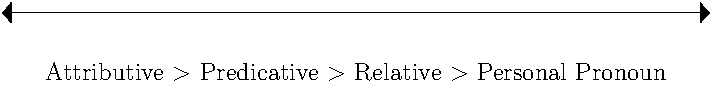
\includegraphics[scale=0.7]{figures/EngerFig1}

\begin{tikzpicture}
\draw[{Latex[width=4mm]}-{Latex[width=4mm]}] (0,1) -- (10,1);
\node (txt) at (5,.5) {\smaller Attributive $>$ Predicative $>$ Relative $>$ Personal Pronoun};
\end{tikzpicture}
\caption{The \isi{Agreement Hierarchy}.}
\label{fig:Enger:agree1}
\end{figure}

%
%Corbett (2006: 207) 
\citet[207]{Corbett2006} %
%Corbett
%
says that for ``any controller that permits
alternative agreements, as we move rightwards along the Agreement
Hierarchy, the likelihood of agreement with greater semantic
justification will increase monotonically''. In other words: The
possibility for semantic agreement will increase towards the right; if
possible on the predicative, it will be possible on the personal pronoun
too, but not necessarily the other way around. A case in point is the
agreement patterns noted for some Scandinavian mass nouns (\sectref{sec:enger:2.4}). Given
that \ili{Danish} allows semantic agreement on the attributive determiner
(\emph{det vodka}), semantic agreement is expected also on the
predicative. In standard \ili{Swedish}, semantic agreement is possible on the
predicative; so, semantic agreement is expected also on personal
pronouns, but it is no problem that semantic agreement is outlawed on
the determiner.

While Corbett's hierarchy was originally  formulated as a synchronic
constraint, it ``can easily be adapted to the diachronic perspective,
predicting \isi{gender} exponents to begin and/or complete the transition from
lexical {[}syntactic{]} to referential {[}semantic{]} assignment the
earlier, the further they are located on the right of the implicational
hierarchy'', as noted by %
%Dolberg (2014: 55)
\citet[55]{Dolberg14}%
%Dolberg
%
.

\subsection{The revised \isi{Agreement Hierarchy}}

\subsubsection{Suggestion and background}
\label{sec:enger:3.2.1}

The suggestion now is to modify the hierarchy, at least for some
purposes, by expanding it with an additional position or `peg', which is
`word-internal', cf. Figure~\ref{fig:Enger:agree2}.


\begin{figure}
%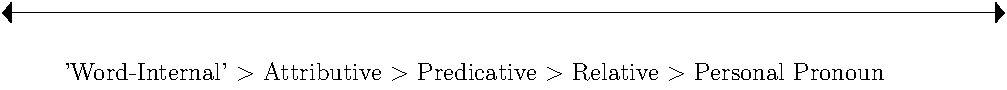
\includegraphics[scale=0.7]{figures/EngerFig2}
\centering
\begin{tikzpicture}
\draw[{Latex[width=4mm]}-{Latex[width=4mm]}] (0,1) -- (10,1);
\node (txt) at (5,.5) {\smaller `Word-Internal' $>$ Attributive $>$ Predicative $>$ Relative $>$ Personal Pronoun};
\end{tikzpicture}
\caption{Modified \isi{Agreement Hierarchy}.}
\label{fig:Enger:agree2}
\end{figure}

%\textbf{`Word-internal'} Attributive Predicative Relative Personal
%pronoun

The idea is that the \isi{Agreement Hierarchy} has to do with `tightness' of
grammatical relations, and thus with \isi{grammaticalisation}, and that
grammatical relations generally are tighter inside the word than inside
the phrase, and tighter inside the phrase than outside it, -- and across
clauses weaker still. The idea that the \isi{Agreement Hierarchy} may have to
do with \isi{grammaticalisation} is far from original %
%(cf. Lehmann 1982, 2016)
\citep[cf.][]{Lehmann82,Lehmann16}%
%Lehmann;Lehmann
%
, but it has not received quite the attention it merits %
%(though see
%Jobin 2004)
\citep[though see][]{Jobin04}%
%Jobin
%
.

When suggesting the hierarchy, %
%Corbett (1979: 217) 
\citet[217]{Corbett79} %
%Corbett
%
noted that it did not
match then-current syntactic frameworks too well, and suggested that it
was an ``independent feature of natural languages''. Nearly forty years
later, this suggestion seems less appealing. As %
%Dolberg (2014: 58)
\citet[58]{Dolberg14}
%Dolberg
%
notes, from a diachronic perspective, Corbett's \isi{Agreement Hierarchy} ``is
to be credited with being of remarkable predictive accuracy, yet it does
not yield much in the way of explanatory power: even though it reliably
tells us what to expect to happen in the exponents of changing \isi{gender}
systems, it provides little information regarding why this is so.''

It would if the \isi{Agreement Hierarchy} could be grounded in something else.
In recent years, many linguists have come to see constraints ``not so
much as constraints on possible synchronic grammars {[}than, HOE{]} as
constraints on diachronic developments'' %
%(Timberlake 2003: 194, cf. also
%e.g. Evans \& Levinson 2009)
(\citealt{Timberlake03}: 194, cf. also e.g. \citealt{Evans2009})%
%\citep[194, cf. also e.g. Evans \& Levinson 2009]{Timberlake03}%
%Timberlake
%
. On such a view, at least some of the
explanatory burden is shifted from synchrony towards diachrony.

According to %
%Lehmann (1982, 2015 and elsewhere)
\citeauthor{Lehmann82} (\citeyear{Lehmann82,Lehmann15} and elsewhere)%
%
%\citet[ and elsewhere]{Lehmann82,Lehmann15}%
%Lehmann;Lehmann
%
, there is a unidirectional movement from semantic agreement towards syntactic
agreement, but not vice versa. In other words, what starts out as
semantic agreement may become `syntacticised' and less meaningful;
changes in the other direction should not occur. Becoming somehow
`semantically reduced' is a standard criterion for \isi{grammaticalisation},
another is becoming more obligatory. Both criteria would seem to hold
for `syntactic' agreement compared to semantic; %
%Wechsler (2009) 
\citet{Wechlser03} %
%Wechsler
%
even
prefers the term `grammatical' agreement. This fits with the broad
picture of \isi{grammaticalisation}; it is largely unidirectional. On the
assumption that diachronic tendencies motivate the \isi{Agreement Hierarchy},
the hierarchy can be related to a larger framework, viz. that of
\isi{grammaticalisation}.

\subsubsection{Objection I: motivating the fifth peg}
\label{sec:enger:3.2.2}
\largerpage
The fifth peg may seem like cheating, for two reasons. Firstly,
`word-internal (or noun-internal) agreement' is a controversial
notion.\footnote{While %
%Stolz (2006) 
\citet{Stolz07} % texte 06, refs 07 dans l'original
%?Stolz
%
argues at length in favour of the
  notion of word-internal agreement, the point I am trying to make here
  is orthogonal to his.} The other `pegs' are syntactic heads; the
\isi{suffix} in Norwegian is morphology (cf. \sectref{sec:enger:2.3}), and the idea of
`morphology-free syntax' is well-established %
%(Zwicky 1992, Corbett 2014)
\citep{Zwicky92,Corbett14}%
%Zwicky;Corbett
%
. Secondly, merely positing a fifth peg does not automatically
solve the problem; the new peg does require some kind of motivation. As
the \isi{Agreement Hierarchy} has already been linked to \isi{grammaticalisation}
(\sectref{sec:enger:3.2.1}), the latter problem will be discussed first.

There are different versions around of the \isi{Agreement Hierarchy}. %
%Köpcke
%et al. (2010) 
\citet{Kopcke10} %
%Köpcke-al.
%
try to make their version less system-internal and more
functional. In the words of %
%Dolberg (2014: 18)
\citet[18]{Dolberg14}%
%Dolberg
%
, they ``assign pragmatic
functions to the syntactic categories identified by Corbett, resulting
in this altered agreement hierarchy\is{Agreement Hierarchy}: specifying -- modifying --
predicating -- referent-tracking''. %
%Dolberg (2014: 58) 
\citet[58]{Dolberg14} %
%Dolberg
%
argues that it
makes sense to consider this version of the hierarchy together with
Corbett's original:

\begin{quote}
[M]otivating this expected pathway of referential agreement encroaching
into (predominantly) lexical \isi{gender} systems is comparably
straightforward in the functional version of the \isi{Agreement Hierarchy}
{[}%
%Köpcke et al. 2010
\citealt{Kopcke10}%
%
{]}, simply by taking recourse to the basic surmise
that changes will occur generally first in those areas, in which the
change is most conducive and/or least detrimental to language use. Thus,
the underlying assumption of the functional version of the Agreement
Hierarchy is that personal pronouns changing to referential \isi{gender} yield
the largest gain in freeing cognitive capacity, as their lexical \isi{gender}
needs no longer be remembered over comparably long stretches of
discourse, because the appropriate pronoun form is now simply being
derived from attributes of the referent, or, more precisely, the
interlocutor's mental representation thereof, which needs to be kept in
working memory anyway. This putative gain then gradually diminishes the
further one moves to the left in the Hierarchy. %
%(Dolberg 2014: 58)
\citep[58]{Dolberg14}%
%Dolberg
%

\end{quote}

Relating the \isi{Agreement Hierarchy} to \isi{grammaticalisation} (cf. \sectref{sec:enger:3.2.1}) means
relating it to the `tightness' of grammatical relations; one of
%
%Lehmann's (2015: 131) 
\citeposp{Lehmann15}{131} %
%Lehmann
%
`parameters' of \isi{grammaticalisation} is bondedness
or `tightness': ``The cohesion of a sign with other signs in a syntagm
will be called its bondedness; this is the degree to which it depends
on, or attaches to, such other signs.'' %
%Lehmann (2015: 157) 
\citet[157]{Lehmann15} %
%Lehmann
%
says the
syntagmatic cohesion or bondedness of a sign ``is the intimacy with
which it is connected with another sign to which it bears a syntagmatic
relation''.

The relation between a noun and an attributive adjective is tighter,
more ``intimate'', than that between a noun and a predicative adjective,
which is in turn tighter than that between a noun and a pronoun.
Elements in attributive position are inside the noun phrase, and the
syntax of the phrase is, as a rule, tighter than that of the clause and
sentence. The relation between a pronoun and its antecedent is typically
`loose', compared with that of determiner to noun, hence, semantic
agreement is more characteristic of pronouns. A related `parameter' for
%
%Lehmann (2015: 131) 
\citet[131]{Lehmann15} %
%Lehmann
%
is that of syntagmatic variability; the possibility
of `shifting around' a sign in its construction. This also fits with the
\isi{Agreement Hierarchy}, and the relation between noun and \isi{suffix} is tighter than any of the
relations in Corbett's original hierarchy. The \isi{suffix} has to occur
immediately to the right of the noun stem; nothing else can intervene.

This fits with the suggestions made by %
%Köpcke et al. (2010) 
\citet{Kopcke10} %
%Köpcke-al.
%
and %
%Dolberg (2014)
\citet{Dolberg14}%
%Dolberg
%
. Pronouns are unlikely to be `stored' in the mental lexicon
together with their controlling noun, and this opens for semantic
agreement. By contrast, it seems likely that suffixes\is{suffixation} are stored with
their controller, as some idioms show. Two set phrases in Norwegian are
\emph{få sparken `}get the sack, be fired' and \emph{gi sparken} `sack,
fire'. The verbs \emph{få} and \emph{gi} mean `get, receive' and `give'
respectively, and they are both very general and frequent, but the noun
\emph{sparken} only rarely occurs outside these two idioms; it is
difficult to ascribe a meaning to \emph{sparken} in isolation. There is
no indefinite singular; there are no plurals. Even if the \isi{suffix}
indicates a masculine noun, there is no noun phrase \emph{*en
spark}.\footnote{Strictly speaking, there is a noun \emph{en spark}
  `kicksled, spark', but it is a homonym, synchronically.} If the whole
\emph{få sparken} were stored, that would weaken the case for saying
that only stem and \isi{suffix} are stored together, but \emph{sparken} can
marginally be found on its own, cf. examples from the web in (\ref{ex:Enger:11}):

\ea\label{ex:Enger:11} Examples of \emph{sparken} without \emph{få}:

\ea \emph{Facebook betyr ikke sparken} `Facebook does not {[}have to{]} mean
the sack'

\ex \emph{dermed ble det sparken} `lit. thereby became it sack; so I was
sacked'

\z
\z

Similar examples include \emph{snurten}, which it hardly makes sense to
translate in isolation; it is mostly known from the idiom \emph{se ikke
snurten av} `not see anything/the least bit of'. This noun does occur
marginally in some other contexts, though, even without negation, cf.~(12), again, examples are taken from the web:

\ea\label{ex:Enger:12} Examples of \emph{snurten} without \emph{ikke} (and without
\emph{av}):

\ea \emph{aldri sett snurten av} `never seen anything of'

\ex \emph{uten å se snurten til} `without seeing anything of'

\ex \ldots{} \emph{kan man skimte snurten av peisen} `\ldots{} can one spot a
little of the fireplace'

\z
\z

Scandinavian diachrony presents at least one example where the \isi{definite}
singular \isi{suffix} has become part of the stem. This is the noun meaning
`world'. \ili{Swedish} has \emph{värld}, \ili{Danish} has \emph{verden} (cf. def.
sg. \emph{världen} vs. \emph{verdenen}). The \ili{Danish} cognate is an
innovation; the old def.\textsc{sg}. \isi{suffix} has become part of the stem.
Pragmatically, this makes sense; for most speakers, there is only one
world (at least most of the time). Istro-Romanian also presents examples
where the plural `\isi{definite} article' has become lexicalised %
%(Maiden 2016d)
\citep{Maiden16d}%
%Maiden
%
. It is difficult to think of an example where the pronoun would
merge with the stem in the same way, also because pronouns do not
typically occur next to a noun (as they occur `instead of a noun').

It is more difficult to come up with examples in which the determiner
must be stored than where the \isi{suffix} must, but there are some. The
phrase \emph{ikke det spøtt} means `not the least', and one might expect
the noun \emph{spøtt} to inflect as a regular neuter would. Yet at least
in my Norwegian, there is no \isi{definite} singular form, nor any plurals.
For \emph{spøtt}, then, it seems the determiner is stored with the
noun.\footnote{Admittedly, dictionaries also mention \emph{et spøtt}.
  But that is unknown to many speakers, and dictionaries tend to strive
  for completeness, sometimes at the expense of actual usage.} An
obvious question is if \emph{ikke} `not' also has to be stored, but
\emph{aldri sett det spøtt} `never seen no nothing' shows it does not
have to.

It probably does not happen often that the pronoun is stored together
with the noun; this probably happens more often with the determiner. It
seems even more likely that suffixes\is{suffixation} be stored with the corresponding
noun (also because suffixes\is{suffixation} are `salient', cf. \sectref{sec:enger:3.2.3} below).\footnote{The
  suggestion that determiner or affix may be stored together with the
  noun does not exclude the idea that generalisations may be made over
  the \isi{gender} or inflection class of a noun %
%(cf. e.g. Conzett 2006)
\citep[cf. e.g.][]{Conzett06}%
%Conzett
%
.}

In \sectref{sec:enger:3.2.1}, we considered an argument in favour of seeing the Agreement
Hierarchy in terms of \isi{grammaticalisation} having to do with `semantic
reduction'. According to %
%Heine (2003: 583)
\citet[583]{Heine2003}%
%
, semantic reduction is the
central factor behind \isi{grammaticalisation}. It is helpful to think of
semantic reduction in terms of reduction of uncertainty (entropy). The
less surprising X is, the less is its information value. Consider now
the examples in (\ref{ex:Enger:13}):

\ea\label{ex:Enger:13} Pronoun and determiner in use

\ea\label{ex:Enger:13a} \gll Bilen står framfor huset. Den er faktisk rosa.\\
Car.\textsc{def}.\textsc{sg}.\textsc{\{m\}} {is (lit. stands)} {in front of} house.\textsc{def}.\textsc{sg}.\textsc{\{n\}}. It.\textsc{m} is
actually pink.\\
\glt `The car is in front of the house. It -- i.e. the car -- is actually
pink.'

\ex\label{ex:Enger:13b} \gll Bilen står framfor huset. Det er faktisk rosa.\\
Car.\textsc{def}.\textsc{sg}.\textsc{\{m\}} {is (lit. stands)} {in front of} house.\textsc{def}.\textsc{sg}.\textsc{\{n\}}. It.\textsc{n} is
actually pink.\\
\glt `The car is in front of the house. It -- i.e. the house -- is actually
pink.'

\ex\label{ex:Enger:13c} \gll Den bilen som står framfor huset, er faktisk rosa.\\
The.\textsc{\{m\}} car.\textsc{def}.\textsc{sg}.\textsc{m} that {is (lit. stands)} {in front of} house.\textsc{def}.\textsc{sg}.\textsc{\{n\}} is
actually pink\\

\z
\z

Recall from \sectref{sec:enger:2.4.1} that Norwegian pronouns can typically also be used as
determiners. In (\ref{ex:Enger:13a}, \ref{ex:Enger:13b}), \emph{den} contrasts with \emph{det}. In (\ref{ex:Enger:13c}),
\emph{den} does not contrast with \emph{det}, since *\emph{det bilen} is
ungrammatical. In other words, the first \emph{den} tells us the speaker
is talking about the car, the last \emph{den} merely tells us that a
masculine or feminine will follow (and that it is a \isi{definite}, specific example). Thus, the information value of \emph{den} is higher when used
pronominally than when used determinatively. Another argument in the
same direction would be that the first (personal pronoun) \emph{den} can
be stressed, but the last (determiner) \emph{den} cannot. This indicates
that in general, the attributive determiner has a lower information
value than the personal pronouns. The \isi{suffix} has an even lower
information value than the determiner %
%(cf. Dahl 2015: 123)
\citep[cf.][123]{Dahl15}%
%Dahl
%
. (Recall that
the \isi{suffix} is also even more `bonded', which is one of %
%Lehmann's 2015
\citeauthor{Lehmann15}'s \citeyear{Lehmann15}%
%
:
131 parameters for \isi{grammaticalisation}.)

\subsubsection{Objection II: Agreement between parts of words?}
\label{sec:enger:3.2.3}
\largerpage[-1]
Patching suffixes\is{suffixation} on to the \isi{Agreement Hierarchy} may seem a bad idea on
theoretical grounds; this might at first glance seem tantamount to
denying the claim that syntax is morphology-free %
%(Zwicky 1992, Corbett
%2014:38f)
\citep[38f]{Zwicky92,Corbett14}%
%Zwicky;Corbett
%
. This is a large issue which cannot be discussed in detail
here, but the lexeme, the line between syntax and morphology, has not
been handed down on tablets of stone; there are `troubles with lexemes',
as argued by %
%Fradin \& Kerleroux (2003)
\citet{Fradin03b}%
%Fradin-Kerleroux
%
, %
%Haspelmath (2011) 
\citet{Haspelmath2011} %
%Haspelmath
%
and many
others. A very influential adherent of lexeme-based models, %
%Matthews (1991: 100)
\citet[100]{Matthews91}%
%
, even says ``it is often the mark of a genuine unit, like
the lexeme, that we have trouble with it!''\footnote{%
%Maiden (2016c)
\citet{Maiden16c}
  argues, on the basis of an impressive set of data taken from dialects
  and diachrony, that \ili{Romanian} ``nouns showing \emph{genus alternans}
  are not a class defined by the agreement behaviour of associated
  words, but \textbf{a class the agreement behaviour of whose associated
  words is dictated by inflexional morphology} {[}boldface mine,
  HOE{]}''. The implications are intriguing. Yet Maiden's analysis has
  also been criticised %
%(by Loporcaro 2016)
\citep[by][]{Loporcaro16}%
%Loporcaro
%
. Anyway, the subject of
  `morphology-free syntax' is too large for this paper.}

There has been some debate over whether the Norwegian \isi{definite} singular
\isi{suffix} should be taken as a marker of \isi{gender} or of inflection class (cf.
2.1), and this also relates to the problem of the delimitation
morphology--syntax. %
%Åfarli \& Lohndal (2015) 
\citet{Afarli15} %
%
argue that the \isi{suffix}
-\emph{a} should count as a marker of \isi{gender} (and not `only' of
inflection class), also in the recent Oslo system described in example \ref{ex:Enger:2}. %
%Åfarli \& Lohndal 
\citeauthor{Afarli15} %
%
are not worried about violating lexicalist
doctrines, and that is surely fair enough, given their theoretical
stand; yet it remains too open, in my view, what the consequences will
be: many things normally not included as `\isi{gender}' will then have to fall
under that label (many inflection classes, for instance). From the
opposite side of the spectrum, %
%Lødrup (2011) 
\citet{Lodrup11} %
%Lødrup
%
squarely rejects analysing
\emph{-a} as a \isi{gender} marker, as it is not an `associated word'. An
in-between course is suggested by
%
%Enger (2004a: 65)
\citet{Enger2004a}%
%Enger
%
, who discusses a system like that in example~(\ref{ex:Enger:1}):

\begin{quote}
If genders\is{gender} are defined only on the basis of word-external agreement, it
seems dubious to treat the \isi{definite} singular \isi{suffix} as an exponent of
\isi{gender}. However, one may wonder if there is any reason for speakers not
to consider the \isi{definite} singular \isi{suffix} a \isi{gender} marker, given that the
correlation with \isi{gender} is perfect. In other words, it seems perverse to
deny that the \isi{definite} singular \isi{suffix} is an exponent of \isi{gender},
\textbf{when there is one and only one \isi{definite} singular \isi{suffix}
associated with each \isi{gender}} {[}emphasis added here{]}. {[}\ldots{}{]}
even if what determines \isi{gender} contrasts is what patterns show up on the
target (and not on the controller), affix contrasts that show up on the
controller and that correspond to \isi{gender} contrasts on targets have to be
considered markers of \isi{gender} as well. \citep[65]{Enger2004a}
\end{quote}

This means taking the \isi{definite} sg. \isi{suffix} as an exponent of \isi{gender} in
the classical Oslo dialect~(1), but not in the present-day one~(2),
since the \isi{suffix} did correlate with \isi{gender} then, but does not do so now.
A possible defence of taking \emph{some} suffixes\is{suffixation} into consideration is that
agreement evidence is less salient; considering agreement evidence
requires more subtle reasoning %
%(cf. also Carstairs-McCarthy 1994: 766)
\citep[cf. also][766]{Carstairs-McCarthy1994}%
%Carstairs-McCarthy
%
.\footnote{%
%Wurzel (1986) 
\citet{Wurzel86} %
%?Wurzel
%
even suggested that, in general, exponents
  on the word itself should count.} There is interesting
psycholinguistic evidence that Norwegian children acquire the suffixes\is{suffixation}
for the \isi{definite} singular much earlier than the \isi{gender} in agreeing words %
%(e.g. Westergaard \& Rodina 2015, 2016)
\citep[e.g.][]{Westergaard15,Westergaard16}
.

However, once the \isi{Agreement Hierarchy} is seen as a product of other
factors, it may become a bit less pressing whether, say, in an
example such as \emph{gutten min} `boy.\textsc{def}.\textsc{sg}\{\textsc{m}\} my.\textsc{m}', the relation
between \emph{gutt} `boy' and \emph{min} `my' and that between
\emph{gutt} and \emph{-en} should both be subsumed under `agreement'.
%Corbett (e.g. 2006)
\citet[e.g.][]{Corbett2006} %
 has presented strong arguments in favour of
including pronouns under the label of agreement: There are important
similarities between pronouns and other elements in the hierarchy, so
that drawing a line at any one specific point at the hierarchy will
entail an arbitrary choice and the loss of worthwhile generalisations.
By the same token, I suggest there are some worthwhile generalisations
to be made by including \emph{some} suffixes\is{suffixation} under the scope of the
\isi{Agreement Hierarchy}. Theories should be about opening doors, not about
closing them. The only reason not to include these suffixes\is{suffixation} would be
substantial empirical evidence showing that they behave very differently
from the predictions of the hierarchy.\footnote{Thanks to Florian
  Dolberg for pointing this out to me.}

In \emph{gutten min}, both \emph{min} and \emph{-en} convey information
about \emph{gutt}. The notion of `\isi{intra-morphological meaning}' can be
useful and productive here %
%(e.g. Carstairs-McCarthy 1994, Maiden 2005,
%Enger 2004a)
\citep[e.g.][]{Carstairs-McCarthy1994,Maiden2005,Enger2004a}%
%Carstairs-McCarthy;Maiden;Enger
%
; the notion that an element of a word may `signal' say, a
particular property of the stem. In (\ref{ex:Enger:1}), \emph{-a} has
\isi{intra-morphological meaning}, signalling the noun's inflection class and
its \isi{gender}. This does not mean that \emph{-a} is an `associated word',
only that it gives information about \isi{gender}. In (\ref{ex:Enger:2}), -\emph{a} also
carries \isi{intra-morphological meaning}, but now signalling inflection class
only, because there is now no \isi{gender} agreement related to it.

\section{The danger of drawing too sharp lines}

\subsection{Automatisation}
\label{sec:enger:4.1}

%
%Lehmann (1982) 
\citet{Lehmann82} %
%Lehmann
%
drew a sharp line between NP-internal and NP-external
agreement. One of %
%Corbett's (2006) 
\citepos{Corbett2006} %
%Corbett
%
arguments against this is that there
can be referential/semantic agreement also inside the NP, and \ili{Danish}
\emph{det vodka} and Norwegian \emph{ei lærer} (cf. \sectref{sec:enger:2.4}) support
Corbett's view. Perhaps paradoxically, if Lehmann is right in arguing
that agreement has to do with \isi{grammaticalisation} (cf. \sectref{sec:enger:3.2.1}), then it is
to be expected that Corbett should be right in not drawing a sharp line.
Grammaticalisation\is{grammaticalisation}  tends to be a gradual affair; I see no reason why it
should come to a complete halt exactly at the NP.

As noted, a development from (feminine) \isi{gender} to inflection class may
be described as \isi{grammaticalisation} (cf. \sectref{sec:enger:2.1}). Grammaticalisation\is{grammaticalisation}  may in
turn be related to automatisation, according to %
%Lehmann (2016)
\citet{Lehmann16}%
%Lehmann
%
.\footnote{There are many suggestions in the literature that are
  similar to that of Lehmann. %
%Boye \& Harder (2012) 
\citet{Boye12} %
%Boye-Harder
%
relate
  \isi{grammaticalisation} to `backgrounding'; automatisation and
  backgrounding are related. %
%Bybee (2003) 
\citet{Bybee03} %
%Bybee
%
relates \isi{grammaticalisation} to
  `chunking'; her explanation of this concept makes it quite clear that
  automation is relevant here too. %
%Haiman (1994) 
\citet{Haiman94} %
%Haiman
%
links
  \isi{grammaticalisation} to ritualization and repetition. %
%Lehmann (2016)
\citet{Lehmann16}  does not address the relation between his suggestion and these others.}
He sees inflectional classes as more `automatised' than genders\is{gender}, and he
says one almost has to be a linguist to wilfully produce the wrong
allophone of a phoneme or to choose the wrong inflectional \isi{suffix}.
Pronominal \isi{gender} is at the other end of the spectrum. It is for
pronouns that there is most `leeway'. They are the least `automatised'.
This perspective fits the one adopted here.

However, under certain circumstances, even inflection class \is{suffix}suffixes can
be manipulated consciously, and not only by linguists. When looking for
examples like \emph{ei lærer} %
%(Section 2.4.2, Enger 2015)
\citep[Section 2.4.2,][]{Enger15}%
%Enger
%
, I found (in a net
forum for `nurse jokes') \emph{ei søt sykepleier} `a.\textsc{f} cute.\textsc{mf} nurse'.
Now, in Norwegian Bokmål, \emph{en søt sykepleier} `a.\textsc{m} cute.\textsc{mf} nurse',
with masculine determiner \emph{en}, is the only conventional choice. In
writing \emph{ei søt sykepleier}, the author emphasises that the nurse
is a woman. Another author on the same net forum reacted to the wording
in an interesting way. Rather than criticise the choice of \emph{ei}
directly, he lists a part of the paradigm, the way it is taught to
school-children, and then comments (my translation and editing) in (\ref{ex:Enger:14}):

\ea\label{ex:Enger:14} {ei sykepleier, sykepleiera}?\\
\glt `Where did you learn your
Norwegian?'
\z

This is an argument \emph{ad absurdum}: if you say A (\emph{ei
sykepleier}), then B (\emph{sykepleiera}) follows, and given that B
(\emph{sykepleiera}) is absurd, A (\emph{ei sykepleier}) must be
rejected. For present purposes, the point of interest is B: Using the
old feminine \isi{suffix} is apparently even worse than the use of feminine
determiner. In short, even if the \isi{suffix} is extremely automatised, it
can be manipulated and changed.

\subsection{Pronouns}
\label{sec:enger:4.2}

\subsubsection{A problem for the present approach?}

%
%Lehmann (1982, 2016) 
\citet{Lehmann82,Lehmann16} %
%Lehmann;Lehmann
%
is not the only linguist who has wished to draw a
sharp line between NP-internal agreement and pronominal agreement. So
far, pronouns have been kept out of the picture, but they are worth
including. In the Oslo dialect today, there are four pronouns. Consider~(\ref{ex:Enger:15}).

\ea\label{ex:Enger:15} Pronouns in the current Oslo dialect

\ea\label{ex:Enger:a} \emph{gutten}.\textsc{m} (the boy) -- \emph{han} `he'

\ex\label{ex:Enger:b} \emph{jenta}.\{?\} (the girl) -- \emph{hun} `she'

\ex \emph{låven}.\textsc{m} (the barn) / \emph{jakka}.\textsc{\{?\}} (the jacket) -- \emph{den}
`it.\textsc{non-neut}'

\ex \emph{barnet}.\textsc{n} (the child) -- \emph{det} `it.\textsc{neut}'

\z
\z

The choice of pronoun relates to animacy. The pronouns \emph{han, hun}
are used with animates (males and females respectively), \emph{den, det}
with non-animates (\emph{den} with non-neuters, \emph{det} with neuters). Animacy does not generally play a role for \isi{gender} agreement
inside the NP in Scandinavian %
%(though cf. Enger 2013: 286--289)
\citep[though cf.][286--289]{Enger13}%
%Enger
%
. Pronoun
agreement and noun-phrase-internal agreement thus follow partly
different rules in this system, as in \ili{Danish} and \ili{Swedish}. Therefore,
some conclude that pronouns are not subject to \isi{gender} agreement %
%(e.g.
%Josefsson 2009, 2014a)
\citep[e.g.][]{Josefsson09,Josefsson14b}%
%Josefsson;Josefsson
%
. An alternative view is that pronouns should be
included under \isi{gender} %
%(e.g. Corbett 2006, Enger 2013, Dolberg 2014,
%Haugen \& Enger 2014, van Epps \& Carling 2017)
\citep[e.g.][]{Corbett2006,Enger13,Dolberg14,Haugen14,VanEpps17}%
%Corbett;Enger;Dolberg;Haugen-Enger
%
.

Once pronouns are taken into account, it may seem that the modified
\isi{Agreement Hierarchy} gets into trouble: It might seem as if the feminine
in Oslo now is retained in the very extremes of the hierarchy, viz. the
pronominal peg and the \isi{suffix} peg, and not in-between. On closer
inspection, however, this is not so. As noted, the \isi{Agreement Hierarchy}
predicts that a new \isi{gender} system, if semantically based, will start
from the right end of the hierarchy and the old system will stay on the
longest at the very left end. The word \emph{hun} in (\ref{ex:Enger:13}) indicates a
human -- or a higher animal -- of female sex. That is not the
\isi{intra-morphological meaning} of -\emph{a} (cf. \sectref{sec:enger:3.2.3}). While the
\isi{intra-morphological meaning}  of -\emph{a} can be roughly given as `the
stem to my left belongs to a particular inflection class, including
words as \emph{jakke} `jacket' and many others', the meaning of
\emph{hun} is roughly `the noun to my left denotes a person of female
sex'.\footnote{The example also illustrates `semantic reduction', cf.
  \sectref{sec:enger:3.2.2}.}

\subsubsection{A problem for another approach}

In their \ili{Swedish} grammar, %
%Holmes \& Hinchliffe (2013: 4) 
\citet[4]{Holmes13} %
%
say that
``Nouns ending in -a {[}in the indefinite sg., thus ending in -an in the
\isi{definite} sg., HOE{]} which denote animals are often treated as feminine
irrespective of their true \isi{gender} {[}i.e. biological sex, HOE{]}:
\emph{råttan} \emph{-- hon} the rat -- she, \emph{åsnan -- hon} the
donkey -- she''.

This observation is interesting, as it represents a problem for an
important approach to Scandinavian \isi{gender}. According to %
%Josefsson (2009:
%40, 2014a)
\citeauthor{Josefsson09} (\citeyear{Josefsson09}: 40, \citeyear{Josefsson14b})%
%\citet[40, 2014a]{Josefsson09}%
%Josefsson
%
, lexical \isi{gender}, which is found within the DP, does not carry
any meaning. By contrast, \isi{gender} is a meaningful category in the
pronominal domain. Thus, Josefsson's approach implies a sharp boundary
between pronominal agreement, which is meaningful, and DP-internal
agreement, which is not. However, if we wish to explain why \ili{Swedish}
\emph{råttan} `the rat' and \emph{åsnan} `the donkey' are more often
referred to with \emph{hon} than, say, \emph{musen} `the mouse' and
\emph{hästen} `the horse', we are stuck with the fact that the former
end in \emph{--a} in the indefinite singular {[}\emph{råtta, åsna}{]},
the latter do not {[}\emph{mus, häst}{]}. Yet `ending in an \emph{-a} in
the indefinite singular' is hardly a meaningful property. (See %
%Haugen \& Enger, forthc.
\citealt{Haugen17}%
%
, for a summary of other arguments against Josefsson's
approach, and further references.)

\section{Conclusions}
\label{sec:enger:5}
I have pointed out a parallel between Oslo Norwegian and Istro-Romanian.
In both cases, the `last redoubt' of the old feminine is a \isi{suffix} on the
noun. The parallel is not coincidental; there are other Scandinavian
examples (cf.  \sectref{sec:enger:2.4}) indicating that the noun's \isi{suffix} is more `resistant'
towards change than are `associated words'. The difference can relate to
a somewhat modified version of the \isi{Agreement Hierarchy} %
%(Corbett 1979,
%2006; Köpcke et al. 2010)
\citep{Corbett79,Corbett2006,Kopcke10}%
%Corbett;Corbett;Köpcke-al.
%
, in which an extra `peg' is added for the
\isi{suffix}. This modification is in line with the spirit of~\citet{Fradin03b}%
; they also note `troubles with lexemes', but they do
not use those problems as arguments against the lexeme as such. Rather
than getting stuck in such problems, we may, for example, utilise the
handy concept of \isi{intra-morphological meaning}  (\sectref{sec:enger:3.2.3}). Following %
%Lehmann (1982)
\citet{Lehmann82}%
%Lehmann
%
, I have argued that relating the \isi{Agreement Hierarchy} to
\isi{grammaticalisation} may be useful, at least for some purposes.

\section*{Acknowledgments}

This paper would never have been written without Martin Maiden's original
    idea. However, I am also much indebted to Florian Dolberg, for very
    thorough comments on a previous version, and to Jenny Audring,
    Bettina Jobin, Briana van Epps, Hélène Giraudo and Rolf Theil for
    suggestions and ideas at different stages. Thanks to audiences in
    Oxford (Nov 2016) and Lund (May 2017). Finally, I have long been
    indebted to Bernard Fradin, for years of generous collegial
    encouragement. It is a pleasure to be able to dedicate this paper to
    him.

%\nocite{Boye12}
%\nocite{Bybee03}
%\nocite{Carstairs-McCarthy1994}
%\nocite{Conzett06}
%\nocite{Conzett11}
%\nocite{Corbett79}
%\nocite{Corbett1991}
%\nocite{Corbett2006}
%\nocite{Corbett2007}
%\nocite{Corbett14}
%\nocite{Corbett16}
%\nocite{Dahl99a}
%\nocite{Dahl99b}
%\nocite{Unterbeck99}
%\nocite{Dahl15}
%\nocite{Dolberg14}
%\nocite{Enger2004a}
%\nocite{Enger2004a}
%\nocite{Enger2004c}
%\nocite{Enger13}
%\nocite{Enger15}
%\nocite{Enger12}
%\nocite{Evans2009}
%\nocite{Fradin03b}
%\nocite{Faarlund09}
%\nocite{Haiman94}
%\nocite{Halmoy16}
%\nocite{Hansen11}
%\nocite{Haspelmath99}
%\nocite{Haspelmath2011}
%\nocite{Haugen14}
%\nocite{Haugen17}
%\nocite{Holmes13}
%\nocite{Jobin04}
%\nocite{Josefsson09}
%\nocite{Josefsson14}
%\nocite{Josefsson14b}
%\nocite{Kopcke10}
%\nocite{Kristoffersen00}
%\nocite{Lahiri05}
%\nocite{Larsen1907}
%\nocite{Ledgeway16}
%\nocite{Ledgeway16b}
%\nocite{Lehmann82}
%\nocite{Lehmann15}
%\nocite{Lehmann16}
%\nocite{Loporcaro16}
%\nocite{Lodrup11}
%\nocite{Lodrup16}
%\nocite{Maiden2005}
%\nocite{Maiden16}
%\nocite{Maiden16b}
%\nocite{Maiden16c}
%\nocite{Maiden16d}
%\nocite{Matthews91}
%\nocite{Opsahl09}
%\nocite{Stolz07}
%\nocite{Timberlake03}
%\nocite{VanEpps17}
%\nocite{Wechlser03}
%\nocite{Wechsler13}
%\nocite{Westergaard15}
%\nocite{Westergaard16}
%\nocite{Wurzel86}
%\nocite{Zwicky92}
%\nocite{Afarli15}

\il{Istro-Romanian|)}
\il{Norwegian|)}

{\sloppy
\printbibliography[heading=subbibliography,notkeyword=this]
}


\end{document}
